\documentclass[10pt]{book}

%These tell TeX which packages to use.
\usepackage{array,epsfig}
\usepackage{amsmath}
\usepackage{amsfonts}
\usepackage{amssymb}
\usepackage{amsxtra}
\usepackage{amsthm}
\usepackage{mathrsfs}
\usepackage{color}
\usepackage{multicol}
\usepackage{enumitem}
%\usepackage{mdframed}
\usepackage[most]{tcolorbox}
\usepackage{pgfplots}
\usetikzlibrary{arrows}
\pgfplotsset{compat=1.6}

\pgfplotsset{soldot/.style={color=black,only marks,mark=*}} \pgfplotsset{holdot/.style={color=black,fill=white,only marks,mark=*}}

%Here I define some theorem styles and shortcut commands for symbols I use often
\theoremstyle{definition}
\newtheorem{defn}{Definition}
\newtheorem{thm}{Theorem}
\newtheorem{cor}{Corollary}
\newtheorem*{rmk}{Remark}
\newtheorem{lem}{Lemma}
\newtheorem*{joke}{Joke}
\newtheorem{ex}{Example}
\newtheorem*{soln}{Solution}
\newtheorem{prop}{Proposition}

\newcommand{\lra}{\longrightarrow}
\newcommand{\ra}{\rightarrow}
\newcommand{\surj}{\twoheadrightarrow}
\newcommand{\graph}{\mathrm{graph}}
\newcommand{\bb}[1]{\mathbb{#1}}
\newcommand{\Z}{\bb{Z}}
\newcommand{\Q}{\bb{Q}}
\newcommand{\R}{\bb{R}}
\newcommand{\C}{\bb{C}}
\newcommand{\N}{\bb{N}}
\newcommand{\M}{\mathbf{M}}
\newcommand{\m}{\mathbf{m}}
\newcommand{\MM}{\mathscr{M}}
\newcommand{\HH}{\mathscr{H}}
\newcommand{\Om}{\Omega}
\newcommand{\Ho}{\in\HH(\Om)}
\newcommand{\bd}{\partial}
\newcommand{\del}{\partial}
\newcommand{\bardel}{\overline\partial}
\newcommand{\textdf}[1]{\textbf{\textsf{#1}}\index{#1}}
\newcommand{\img}{\mathrm{img}}
\newcommand{\ip}[2]{\left\langle{#1},{#2}\right\rangle}
\newcommand{\inter}[1]{\mathrm{int}{#1}}
\newcommand{\exter}[1]{\mathrm{ext}{#1}}
\newcommand{\cl}[1]{\mathrm{cl}{#1}}
\newcommand{\ds}{\displaystyle}
\newcommand{\vol}{\mathrm{vol}}
\newcommand{\cnt}{\mathrm{ct}}
\newcommand{\osc}{\mathrm{osc}}
\newcommand{\LL}{\mathbf{L}}
\newcommand{\UU}{\mathbf{U}}
\newcommand{\support}{\mathrm{support}}
\newcommand{\AND}{\;\wedge\;}
\newcommand{\OR}{\;\vee\;}
\newcommand{\Oset}{\varnothing}
\newcommand{\st}{\ni}
\newcommand{\wh}{\widehat}
%Pagination stuff.
\setlength{\topmargin}{-0.75in}
\setlength{\oddsidemargin}{0in}
\setlength{\evensidemargin}{0in}
\setlength{\textheight}{9.in}
\setlength{\textwidth}{6.5in}
\pagestyle{empty}
\begin{document}
\begin{flushleft}
Name:\underline{\hspace{13cm}}Date:\underline{\hspace{2cm}}
\end{flushleft}
\begin{center}
{\Large Math 1041-012 \hspace{0.5cm} Section 5.2}
\end{center}
%\vspace{0.2 cm}

\begin{tcolorbox}
\subsection*{Definition}
If $f$ is defined on an interval $[a,b]$ then divide the interval into $n$ number of \underline{\hspace{4cm}} with width $\displaystyle \Delta x=\frac{b-a}{n}$, let $x_i^*$ be a sample point in each subinterval.

Then the \underline{\hspace{8cm}} is given by
\[
\int_a^b f(x)\ dx=\lim_{n\rightarrow\infty}\sum_{i=1}^n f(x_i^*)\Delta x=\textrm{ limit sum of rectangle areas}.
\]
If this limit exists for every choice of sample points, then $f$ is \underline{\hspace{3cm}} on $[a,b]$.
\end{tcolorbox}
\begin{figure}[h!]
    \centering
    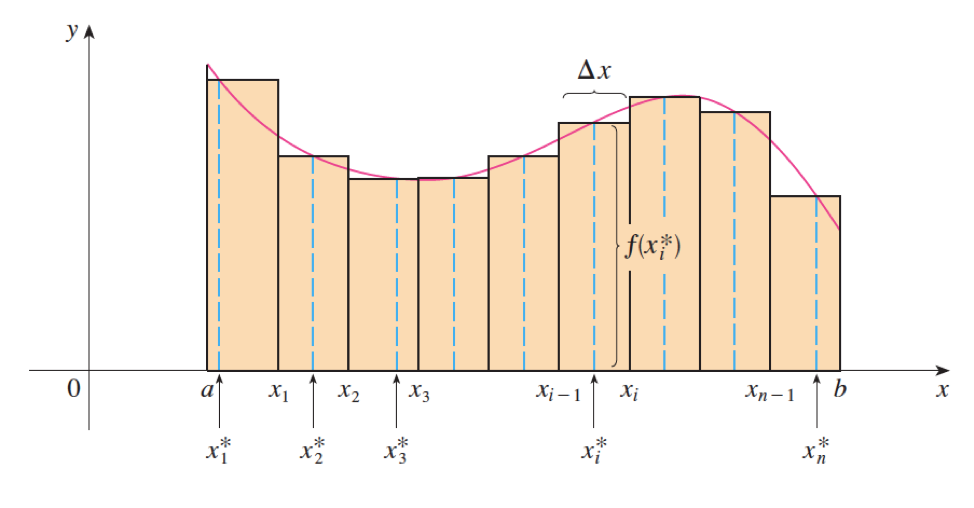
\includegraphics[width=4in]{intRect.png}
\end{figure}
\noindent As we keep \textit{squeezing} more rectangles into the interval we get better approximations to the \underline{\hspace{3cm}} under the curve.
\begin{figure}[h!]
    \centering
    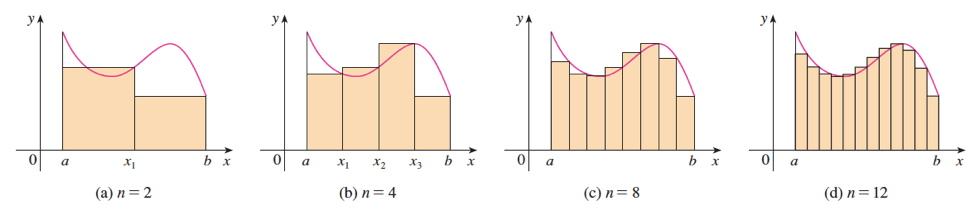
\includegraphics{rect2.png}
\end{figure}\\
\noindent\rule{\textwidth}{1pt}
\begin{figure}[h!]
    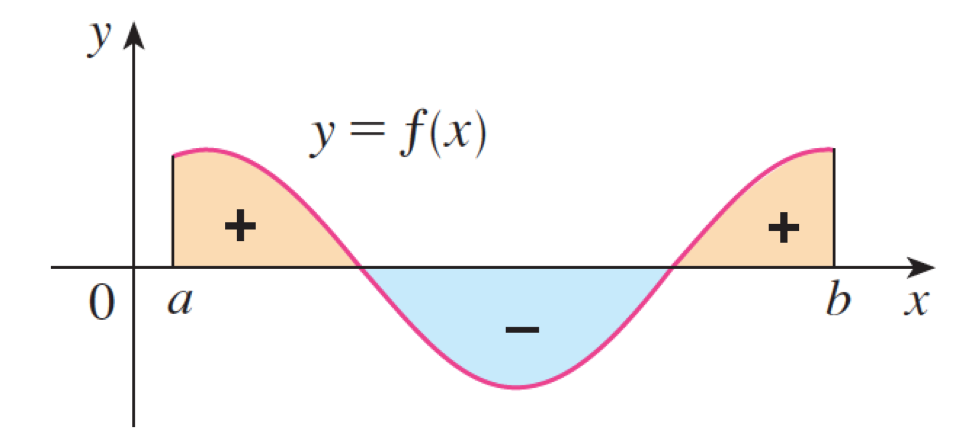
\includegraphics[width=2.5in]{signedarea.png}
\end{figure}
\clearpage
\subsection*{Example 1: Using Areas of known shapes} Evaluate the following integrals by interpreting each in terms of areas.
\begin{multicols}{2}
    \begin{enumerate}[label=(\alph*)]
        \item $\displaystyle\int_0^1\sqrt{1-x^2}\ dx$
        \item $\displaystyle\int_0^3 (x-1)\ dx$ 
    \end{enumerate}
    \end{multicols}
    \vspace{8cm}
\begin{tcolorbox}
\subsection*{Basic Properties of Integrals}
If $a<b$ and $c$ is between $a$ and $b$ then
\begin{itemize}
    \item $\displaystyle \int_a^b K\ dx=K(a-b)$ where $K$ is any constant.
    \item $\displaystyle \int_a^b f(x)\ dx=-\int_b^a f(x)\ dx$,  change direction of integration means change sign.
    \item $\displaystyle\int_a^a f(x)\ dx=0$
    \item $\displaystyle \int_a^b Kf(x)\ dx=K\int_a^b f(x)\ dx$ where $K$ is any constant.
    \item $\displaystyle\int_a^b f(x)+ g(x)\ dx=\int_a^b f(x)\ dx+\int_a^b g(x)\ dx$, integral of sum is sum of integrals
    \item $\displaystyle\int_a^b f(x)- g(x)\ dx=\int_a^b f(x)\ dx-\int_a^b g(x)\ dx$
    \item $\displaystyle \int_a^b f(x)\ dx=\int_a^c f(x)\ dx+\int_c^b f(x)\ dx$, split an integral  when you split interval.
\end{itemize}
\end{tcolorbox}
\clearpage
\subsection*{Example 2: Using a Graph}
The graph of $f(x)$ is shown. Evaluate each integral by interpreting it in terms of areas.
\begin{figure}[h!]
    \centering
    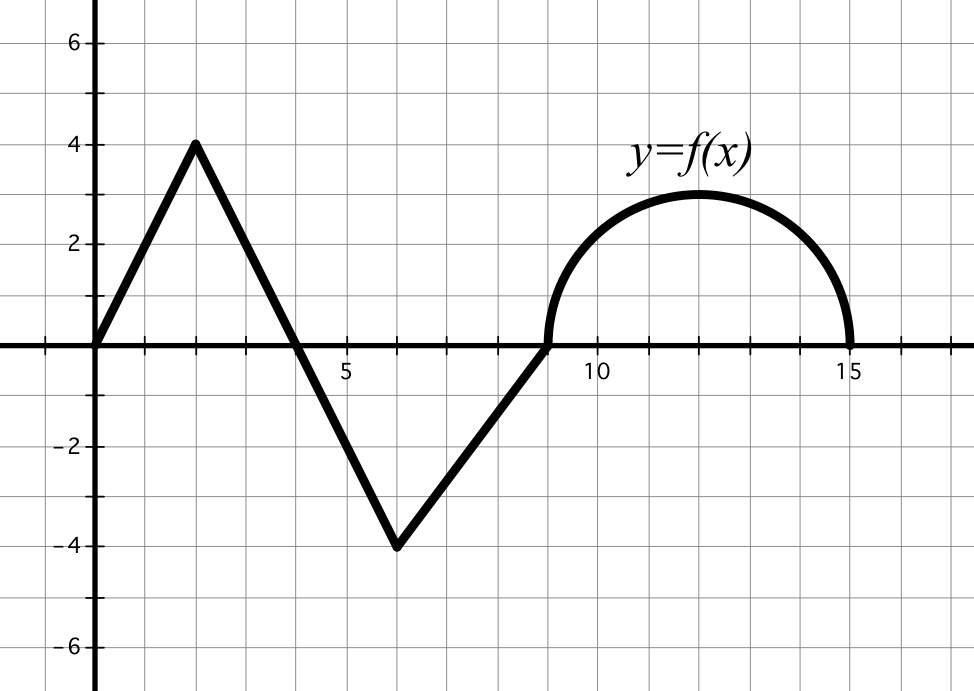
\includegraphics[width=3.5in]{signedareaEx1.png}
\end{figure}
\begin{multicols}{2}
    \begin{enumerate}[label=(\alph*)]
        \item $\displaystyle\int_0^2 f(x)\ dx$\vspace{1.5cm}
        \item $\displaystyle\int_0^4 f(x)\ dx$\vspace{1.5cm} \item $\displaystyle\int_2^6 f(x)\ dx$\vspace{1.5cm}
        \item $\displaystyle\int_0^6 f(x)\ dx$\vspace{1.5cm}
        \item $\displaystyle\int_6^0 f(x)\ dx$\vspace{1.5cm}
        \item $\displaystyle\int_6^9 f(x)\ dx$\vspace{1.5cm}
        \item $\displaystyle\int_9^{12} f(x)\ dx$\vspace{1.5cm}
        \item $\displaystyle\int_0^{12} f(x)\ dx$\vspace{1.5cm}
        \item $\displaystyle\int_4^9 f(x)+3\ dx$\vspace{1.5cm}
        \item $\displaystyle\int_0^9 2f(x)\ dx$\vspace{1.5cm}
    \end{enumerate}
    \end{multicols}
\clearpage
\subsection*{Example 3: U Try}
The graph of $f(x)$ is shown. Evaluate each integral by interpreting it in terms of areas.
\begin{figure}[h!]
    \centering
    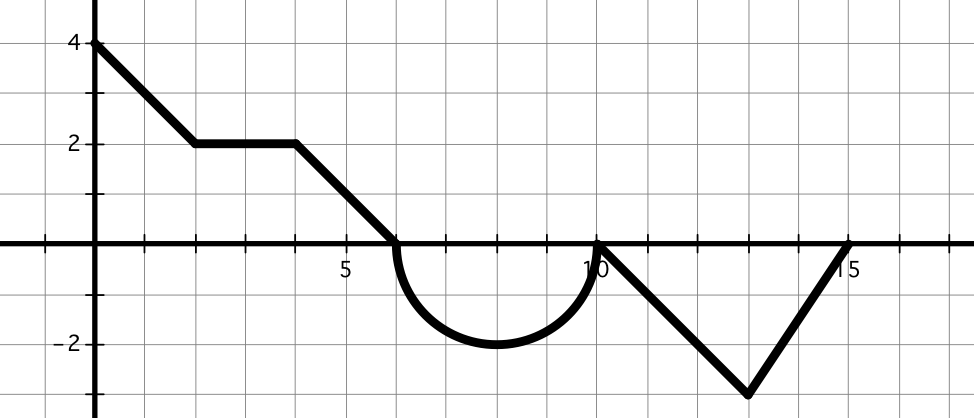
\includegraphics[width=3.5in]{signedareaEx2.png}
\end{figure}
\begin{multicols}{2}
    \begin{enumerate}[label=(\alph*)]
        \item $\displaystyle\int_0^2 f(x)\ dx$\vspace{1.5cm}
        \item $\displaystyle\int_0^4 f(x)\ dx$\vspace{1.5cm} \item $\displaystyle\int_2^6 f(x)\ dx$\vspace{1.5cm}
        \item $\displaystyle\int_0^6 f(x)\ dx$\vspace{1.5cm}
        \item $\displaystyle\int_6^{10} f(x)\ dx$\vspace{1.5cm}
        \item $\displaystyle\int_4^6 f(x)\ dx$\vspace{1.5cm}
        \item $\displaystyle\int_{10}^{15} f(x)\ dx$\vspace{1.5cm}
        \item $\displaystyle\int_0^{12} f(x)\ dx$\vspace{1.5cm}
        \item $\displaystyle\int_4^{10} f(x)+5\ dx$\vspace{1.5cm}
        \item $\displaystyle\int_0^{10} 2f(x)\ dx$\vspace{1.5cm}
    \end{enumerate}
    \end{multicols}
\end{document}